\chapter{\heiti 快速入门}
%\pagestyle{plain}
\pagenumbering{arabic}
\fancypagestyle{plain}
{
\fancyhf{}
\renewcommand{\headrulewidth}{2.4pt}
\renewcommand{\footrulewidth}{2.4pt}
\lhead{
    \setlength{\unitlength}{1mm}
    \begin{picture}(0,0)
    \put(0,0){
\includegraphics[width=0.9cm]{logo.eps}}
    \end{picture}
    }
\chead{}
\rhead{\xiaosi{合肥量子精密仪器有限公司}}
\fancyfoot[LO,RE]{\xiaosi{ASG-GT50-C用户手册}}
\cfoot{}
\fancyfoot[RO,LE]{\xiaosi\textbf{\thepage}}
}


\pagestyle{fancy}
\renewcommand{\headrulewidth}{1.5pt}
\renewcommand{\footrulewidth}{1.5pt}
\lhead{
    \setlength{\unitlength}{1mm}
    \begin{picture}(0,0)
    \put(0,0){
\includegraphics[width=0.9cm]{logo.eps}}
    \end{picture}
    }
\chead{}
\rhead{\xiaosi{合肥量子精密仪器有限公司}}
\fancyfoot[LO,RE]{\xiaosi{ASG-GT50-C用户手册}}
\cfoot{}
\fancyfoot[RO,LE]{\xiaosi\textbf{\thepage}}


\setcounter{page}{1}
\setmainfont{Times New Roman}
\section{\heiti 检查运输}
如运输包装已损坏,请保留被损坏的包装或防震材料,直到货物经过检查且仪器通过电性和机械测试。

\section{\heiti 检查运输包装}
如仪器存在机械损坏或缺失,或者仪器未通过性能测试,请您及时与我司联系。

\section{\heiti 检查随机箱附件}
请根据装箱单检查随机箱附件,随机箱附件包括电源适配器一个,USB连接线一根。如有损坏或缺失,请您及时与我司联系。


\section{\heiti 外观尺寸}
ASG-GT50-C的外观与尺寸如图1.1(仪器前面板)、图1.2(仪器后面板)、图1.3(仪器侧面板)所示,单位为mm。
\begin{figure}[ht]
\centering
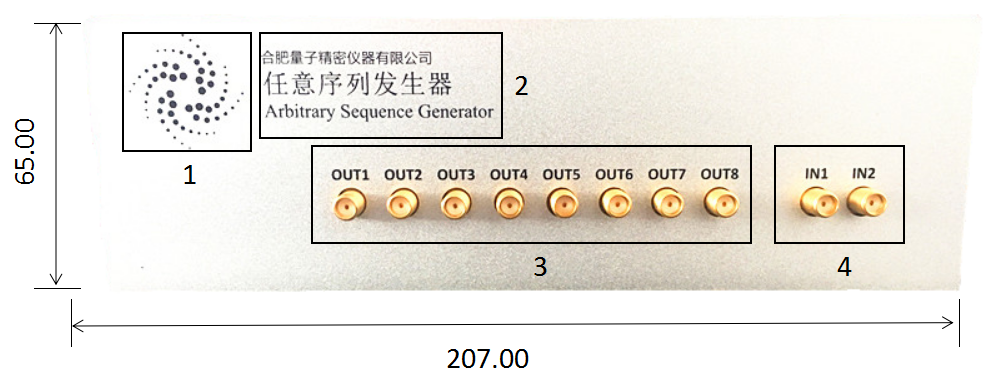
\includegraphics[width=14cm,height=6.5cm]{fig1_1}
\caption{仪器前面板}\label{fig:fig1_1}
%\caption{\textbf{仪器前面板}}\label{fig:fig1_1}
\end{figure}
%\begin{enumerate}
%\item 合肥量子精密仪器有限公司注册商标。
%\item 公司名称与产品名称。
%\item 共 8 个方波输出通道。
%\item “IN1”为保留通道, 用于客户定制化功能; “IN2”为计数信号输入通道。
%\end{enumerate}

\noindent \textbf{1.} 合肥量子精密仪器有限公司注册商标。\\
\textbf{2.}  公司名称与产品名称。\\
\textbf{3.}  共 8 个方波输出通道。\\
\textbf{4.}  其中“IN1”为客户定制化功能通道;“IN2”为计数信号输入通道。

\newpage
\begin{figure}[ht]
\centering
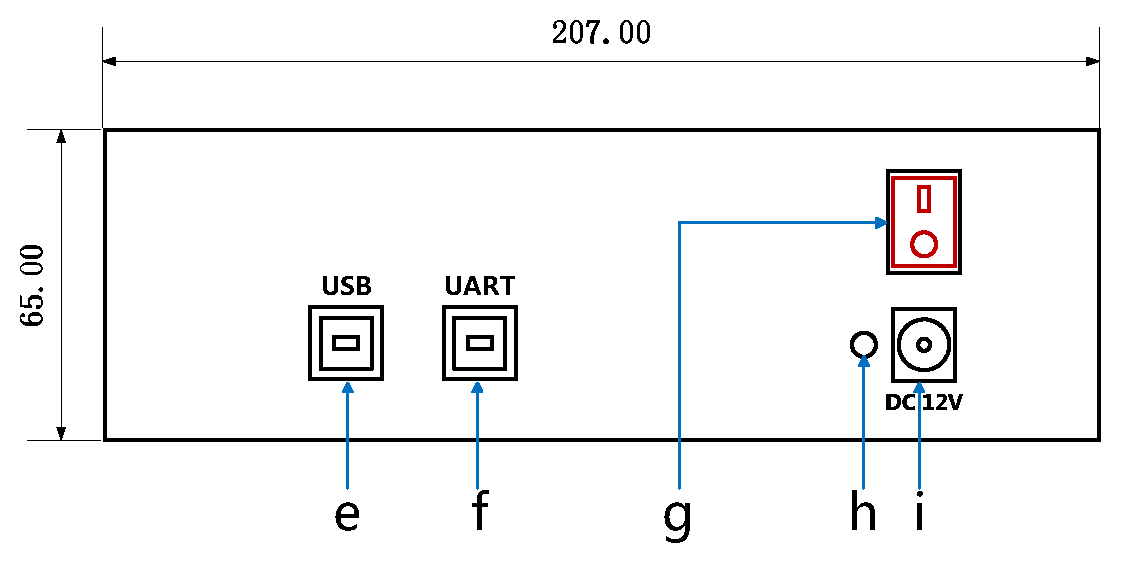
\includegraphics[width=14cm,height=6cm]{fig1_2}
\caption{仪器后面板}\label{fig:fig1_2}
\end{figure}
%\begin{enumerate}
%\item USB通信接口,通过USB连接线将仪器连接到计算机。
%\item “UART”为保留接口,用于客户定制化功能。共8个方波输出通道。
%\item 仪器开关按钮,“I”状态为开,“O”状态为关。
%\item 指示灯,仪器处于工作状态时亮起。
%\item 电源接口。
%\end{enumerate}

\noindent \textbf{1.} USB 通信接口,通过 USB 连接线将仪器连接到计算机。\\
\textbf{2.} 其中“UART”为保留接口,用于客户定制化功能。\\
\textbf{3.} 仪器开关按钮。\\
\textbf{4.} 指示灯,仪器工作时亮起。\\
\textbf{5.} 电源接口。

\begin{figure}[ht]
\centering
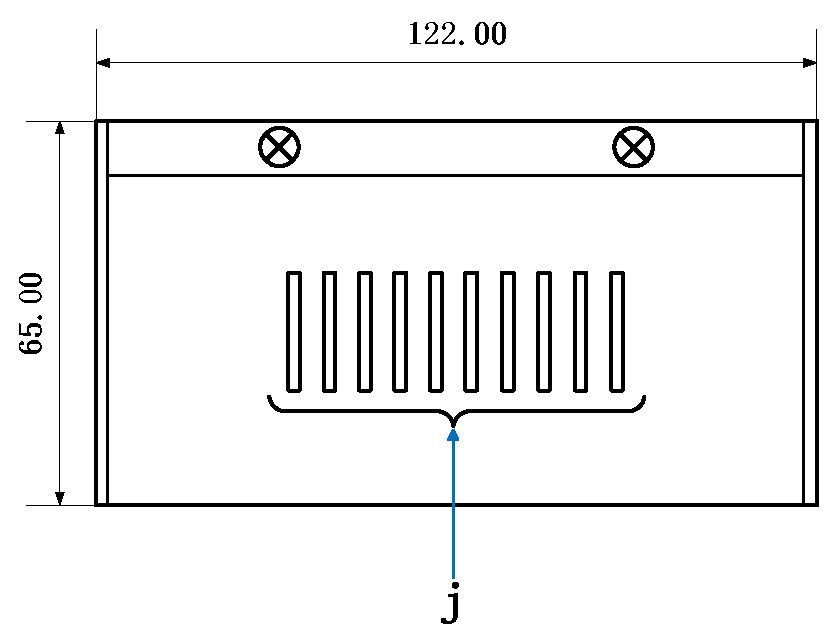
\includegraphics[width=11.6cm,height=6.5cm]{fig1_3}
\caption{仪器侧面板}\label{fig:fig1_3}
\end{figure}
%\begin{enumerate}
%\item 仪器通风口,用于仪器电路板散热。
%\end{enumerate}
\noindent \textbf{1.} 仪器通风口,用于仪器电路板散热。


\section{\heiti 连接电源}
ASG-GT50-C的供电电压为直流12 V。用户可以使用直流稳压电源提供12 V直流电压,或使用随机箱附件提供的电源适配器将仪器连接至220 V,50 Hz的交流电源中。接通电源后,按下开关按钮,可以看到后面板的指示灯亮起,表示仪器已经处于工作状态。

